\documentclass[14pt]{matmex-diploma-custom}

\usepackage{graphicx}
\usepackage{subfigure}

\begin{document}
\filltitle{ru}{
  chair = {Программная инженерия},
  title = {Система сбора и анализа показателей жизнедеятельности на основе данных с мобильных устройств},
  type = {bachelor},
  position = {студента},
  group = 471,
  author = {Байгельдин Александр Юрьевич},
  supervisorPosition = {к.\,ф.-м.\,н., доцент},
  supervisor = {Романовский К.\,Ю.},
  reviewerPosition = {Зам. ген. директора ООО ``ПитерСофтвареХаус''},
  reviewer = {Хитров Д.\,В.},
  year = {2018}
}
\filltitle{en}{
  chair = {Software Engineering},
  title = {System for collection and analysis of vital factors based on data from mobile devices},
  author = {Aleksandr Baigeldin},
  supervisorPosition = {assistant professor},
  supervisor = {Konstantin Romanovsky},
  reviewerPosition = {Deputy director general of ``PiterSoftwareHouse'' Ltd.},
  reviewer = {Denis Khitrov},
  university = {Saint Petersburg State University},
}
\maketitle
\tableofcontents

\section*{Введение}
Стресс --- это совокупность неспецифических (т.е. независимых от типа стрессора)
адаптационных реакций организма на воздействие различных неблагоприятных
факторов (физических или психологических), нарушающих его гомеостаз (стабильное,
равновесное состояние) \cite{book:stress_of_life}. В современной медицине
принято разделять понятие положительного стресса (эустресса) и отрицательного
стресса (дистресса) \cite{article:eustress_distress}. В результате
положительного стресса повышается функциональный резерв организма, происходит
его адаптация к стрессовому фактору и ликвидация самого стресса. Однако, когда
организм постоянно подвергается стрессу или же стрессор слишком сильный,
защитные силы организма истощаются и он становится не в состоянии самостоятельно
справиться со стрессом. От такого стресса страдает иммунная система, он
подрывает здоровье человека и может привести к тяжелым заболеваниям, таким как
депрессивное расстройство, диабет и даже рак \cite{article:stress_and_illness}.
В связи с этим, получили широкое развитие различные методы управления стрессом,
которые помогают предупреждать его отрицательное воздействие. Однако, зачастую
человек не замечает или не осознает того, что подвергается воздействию стресса.
Поэтому перспективной областью исследования является автоматическое отслеживание
стресса в повседневной жизни в реальном времени.

Поскольку основное воздействие стресс оказывает на нервную и эндокринную системы
организма, то для его определения логичным является поиск соответствующих
паттернов в работе этих систем. Например, анализ крови может выявить повышенное
содержание кортизола (глюкортикоидного ``гормона стресса'') в крови. Однако,
инвазивные методы не подходят для непрерывного отслеживания стресса. В связи с
этим, особый интерес вызывает реакция нервной системы организма на стресс, а
если точнее, то реакция симпатического отдела автономной нервной системы,
который отвечает за мобилизацию сил организма в экстренных ситуациях.
Симпатическая нервная система оказывает влияние на частоту сердцебиения и
дыхания, кровяное давление, электрическую активность кожи и другие показатели.
Поэтому диапазон медицинских сенсоров, с помощью которых можно в той или иной
мере определять стресс, довольно обширен: пульсометры, тонометры, GSR сенсоры, и
т.д. Тем не менее, наиболее перспективным типом сенсоров для задачи отслеживания
стресса в реальном времени кажутся именно пульсометры, т.к. несмотря на
небольшую цену, они обладают необходимой мобильностью и предоставляют
возможность высчитывать один из самых важных показателей активности
симпатической нервной системы --- вариабельность сердечного ритма
\cite{article:hrv_stress}.

Однако, симпатическая нервная система реагирует даже на небольшие стрессоры,
которые нет смысла учитывать в статистике, но которые при этом оказывают влияние
на вариабельность сердечного ритма. Например, даже при медленной ходьбе
вариабельность сердечного ритма отличается от сидячего положения
\cite{article:hrv_reliability}, хотя нельзя назвать ходьбу стрессом в
отрицательном смысле. Поэтому учет физической активности (например, на основе
данных с акселерометра) является хорошим способом отфильтровать ложные
срабатывания отслеживающей стресс системы. Для комбинации показателей физической
активности и показателей активности симпатической нервной системы при
определении стресса можно применить популярное на сегодняшний день в медицине
машинное обучение.

Таким образом, для задачи автоматического отслеживания стресса в реальном
времени требуется система, которая бы определяла стресс на основе данных с
пульсометра и акселерометра и обладала бы достаточной мобильностью для того,
чтобы применять ее в повседневной жизни.
	
\section{Постановка задачи}
Целью данной работы является создание прототипа мобильного приложения,
отслеживающего человеческий стресс в реальном времени, определяя его на основе
данных полученных с акселерометра мобильного телефона и внешнего пульсометра,
применяя для этого машинное обучение.

Для достижения этой цели были поставлены следующие задачи:

\begin{itemize}
\item Ознакомиться с природой человеческого стресса и изучить публикации на тему
  определения стресса на основе медицинских данных.
\item Спроектировать архитектуру приложения и его взаимодействия с медицинскими
  сенсорами и моделью машинного обучения.
\item Написать мобильное приложение для сбора данных и выделения из них
  признаков, полезных для определения стресса.
\item Выбрать способ сбора данных, натренировать модель на собранных данных,
  оценить ее эффективность и интегрировать ее в приложение, чтобы достичь
  определения стресса в реальном времени.
\end{itemize}

\section{Обзор}
\subsection{Физиология стресса}
Вегетативная нервная система — это отдел нервной системы, регулирующий
деятельность внутренних органов, который в свою очередь делится на симпатический
и парасимпатический отделы. Парасимпатическая стимуляция одних органов оказывает
тормозное действие, а других — возбуждающее. То же касается и симпатической
симуляции, но в большинстве случаев действие парасимпатической и симпатической
систем противоположно. В частности, парасимпатическая система отвечает за
приведение тела в гомеостаз, ...

При активации симпатической системы, в крови увеличивается содержание кортизола
и глюкозы (гипоталамо-гипофизарно-надпочечниковая система, HPA axis), учащается
частота дыхания, пульс, изменяется электрическая проводимость кожи, ...

Для определения стресса по эндокринной системе, можно применять тесты на
альфа-амилазу, кортизол, ...

Для определения стресса по активности симпатической нервной системы, полезными
оказываются ECG, EMG, GSR сенсоры, ...

Вариабельность сердечного ритма (HRV) — это важный показатель, который отражает
баланс нервной системы и уровень накопленного стресса, ...

HRV можно применять для определения как хронического, так и ситуативного
стресса, ...

\subsection{Существующие решения}

В работе ``Stress Detection Using Low Cost Heart Rate Sensors''
\cite{article:cheap_hrm} не учтена физическая активность.

В работе ``Modeling perceived stress via HRV and accelerometer sensor streams''
\cite{article:accelerometer_hrv} не учтены базовые значения и наивный способ
вычисления физической активности.

...

\section{Архитектура}
\subsection{Инструменты}
В качестве основного языка был выбрал TypeScript, т.к. в отличие от JavaScript
он обладает большими возможностями для рефакторинга благодаря системе типов, ...

Библиотека MedM DeviceKit SDK используется для получения данных с медицинских
сенсоров, ...

React Native используется для написания кроссплатформенного приложения, которое
тем не менее является нативным для обоих платформ, ...

Для написания моста между MedM DeviceKit SDK и React Native используются языки
Kotlin и Swift, ...

MobX используется для управления состоянием приложения в реактивном стиле, ...

D3 используется для упрощения рисования SVG графиков, ...

Python и библиотека SciKit-Learn используются для тренировки модели, ...

\subsection{Взаимодействие с сенсорами}
Разбиение потоков на чанки и сэмплы, ...

Индекс активности (формула) \cite{article:activity_index}, ...

Варибальность сердечного ритма и RMSSD (формула), ...

\subsection{Взаимодействие с моделью}
Сериализация параметров модели, ...

Вычисление пороговых значений для нормализации, ...

Портирование модели в JavaScript \cite{library:sklearn_porter}, ...

Пересчет сэмплов на основе сохраненных данных, ...

\section{Мобильное приложение}
\subsection{Интерфейс}
Управление сенсорами (рис. ~\ref{screenshot:sensors}) было реализовано так,
потому что ...

Настройки и способ калибровки (рис. ~\ref{screenshot:settings}) были реализованы
так, потому что ...

Отображение статистики (рис. ~\ref{screenshot:stats}) было реализовано так,
потому что ...

Экран разработчика (рис. ~\ref{screenshot:dev}) был реализован так, потому что
...

\begin{figure}[ht!]
  \begin{center}
    \subfigure[Экран управления сенсорами]{
      
\includegraphics[width=0.4\textwidth]{images/sensors.png}
      \label{screenshot:sensors}
    } \subfigure[Экран настроек]{
      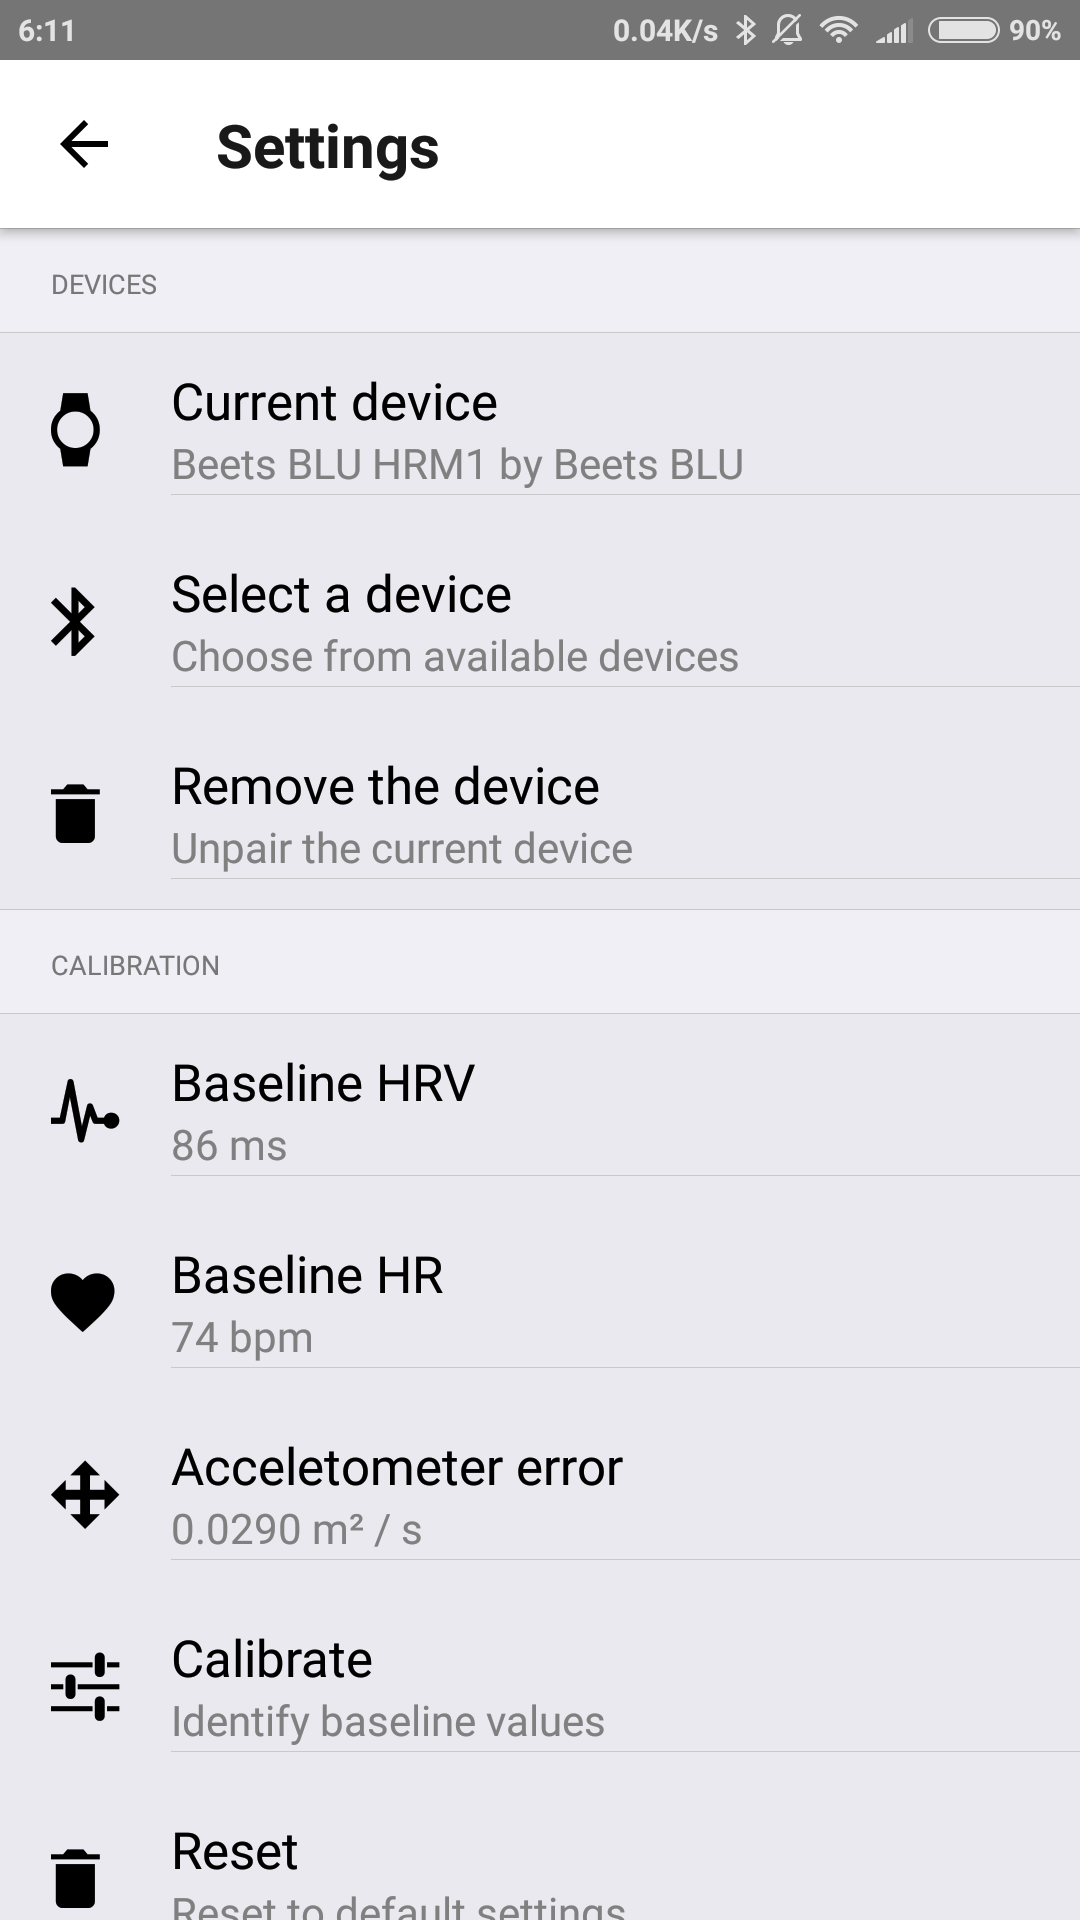
\includegraphics[width=0.4\textwidth]{images/settings.png}
      \label{screenshot:settings}
    } \subfigure[Экран статистики]{
      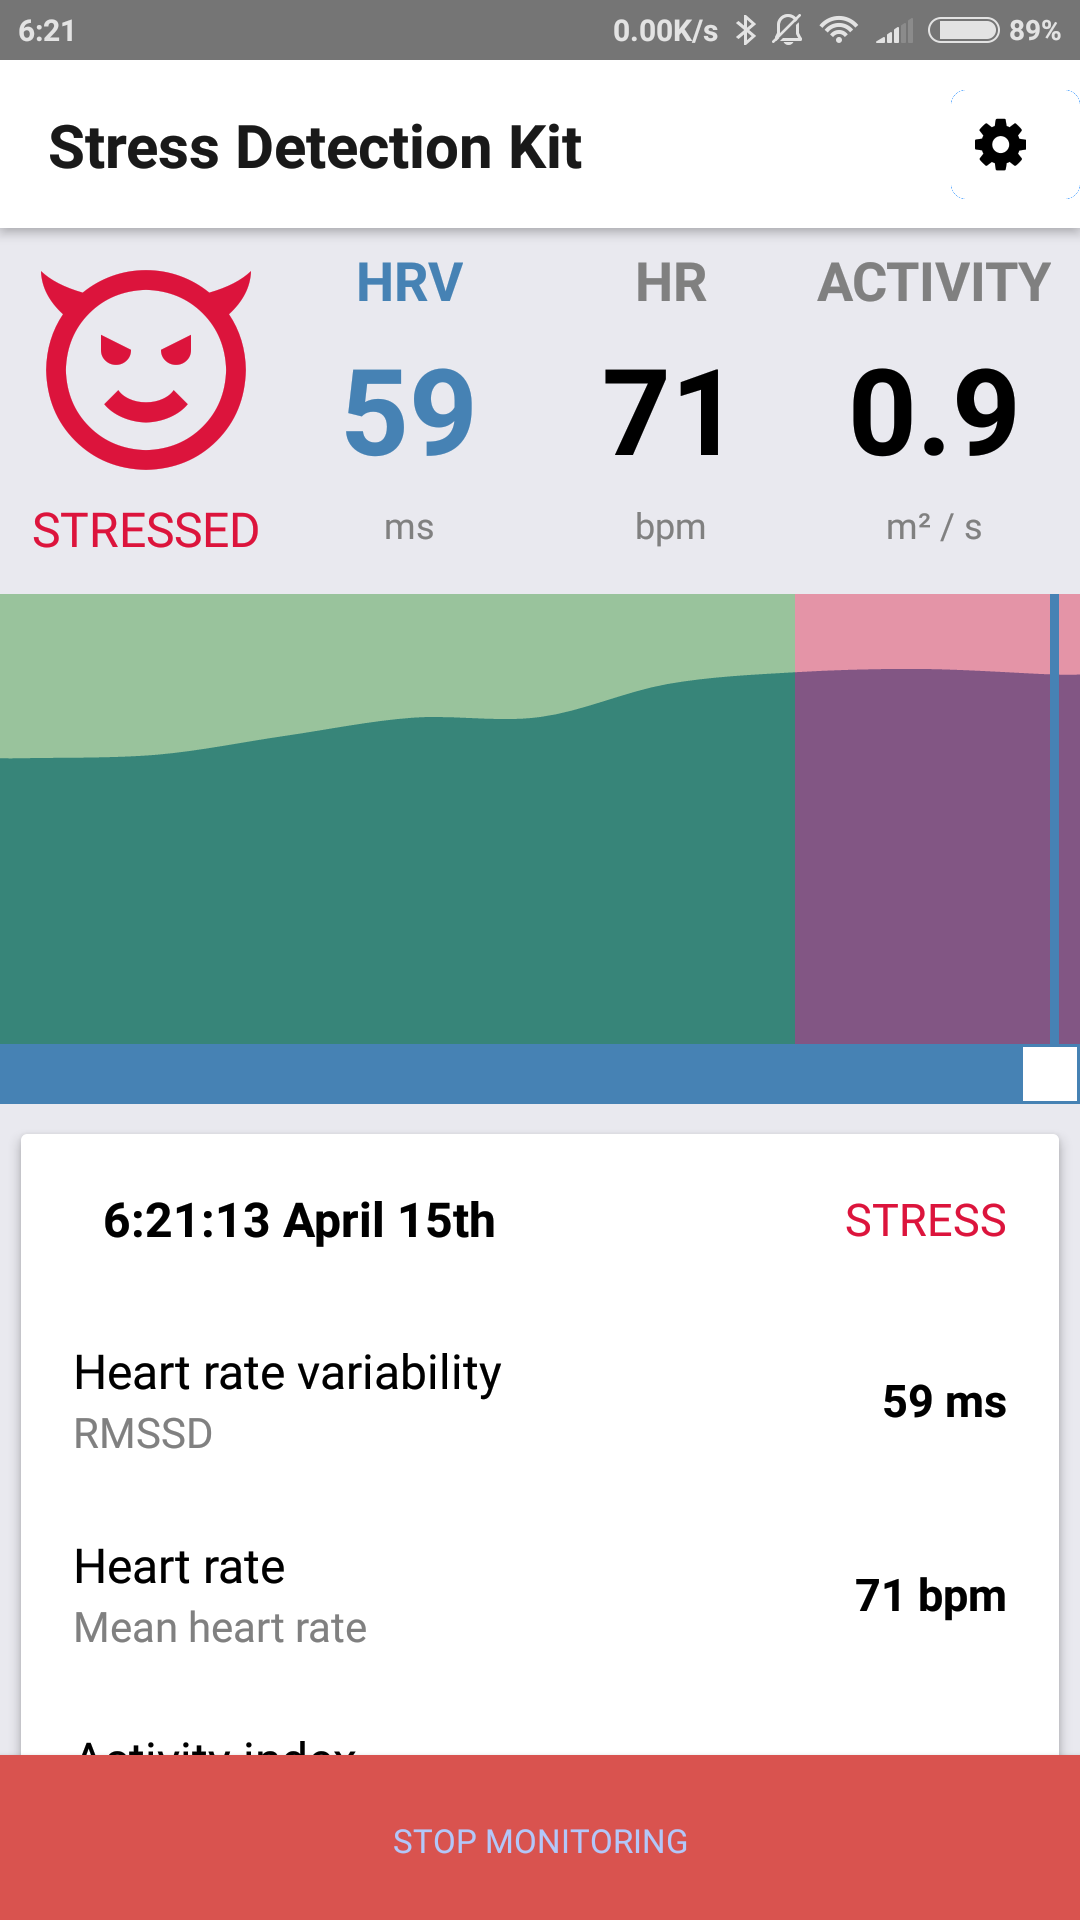
\includegraphics[width=0.4\textwidth]{images/stats.png}
      \label{screenshot:stats}
    } \subfigure[Экран разработчика]{
      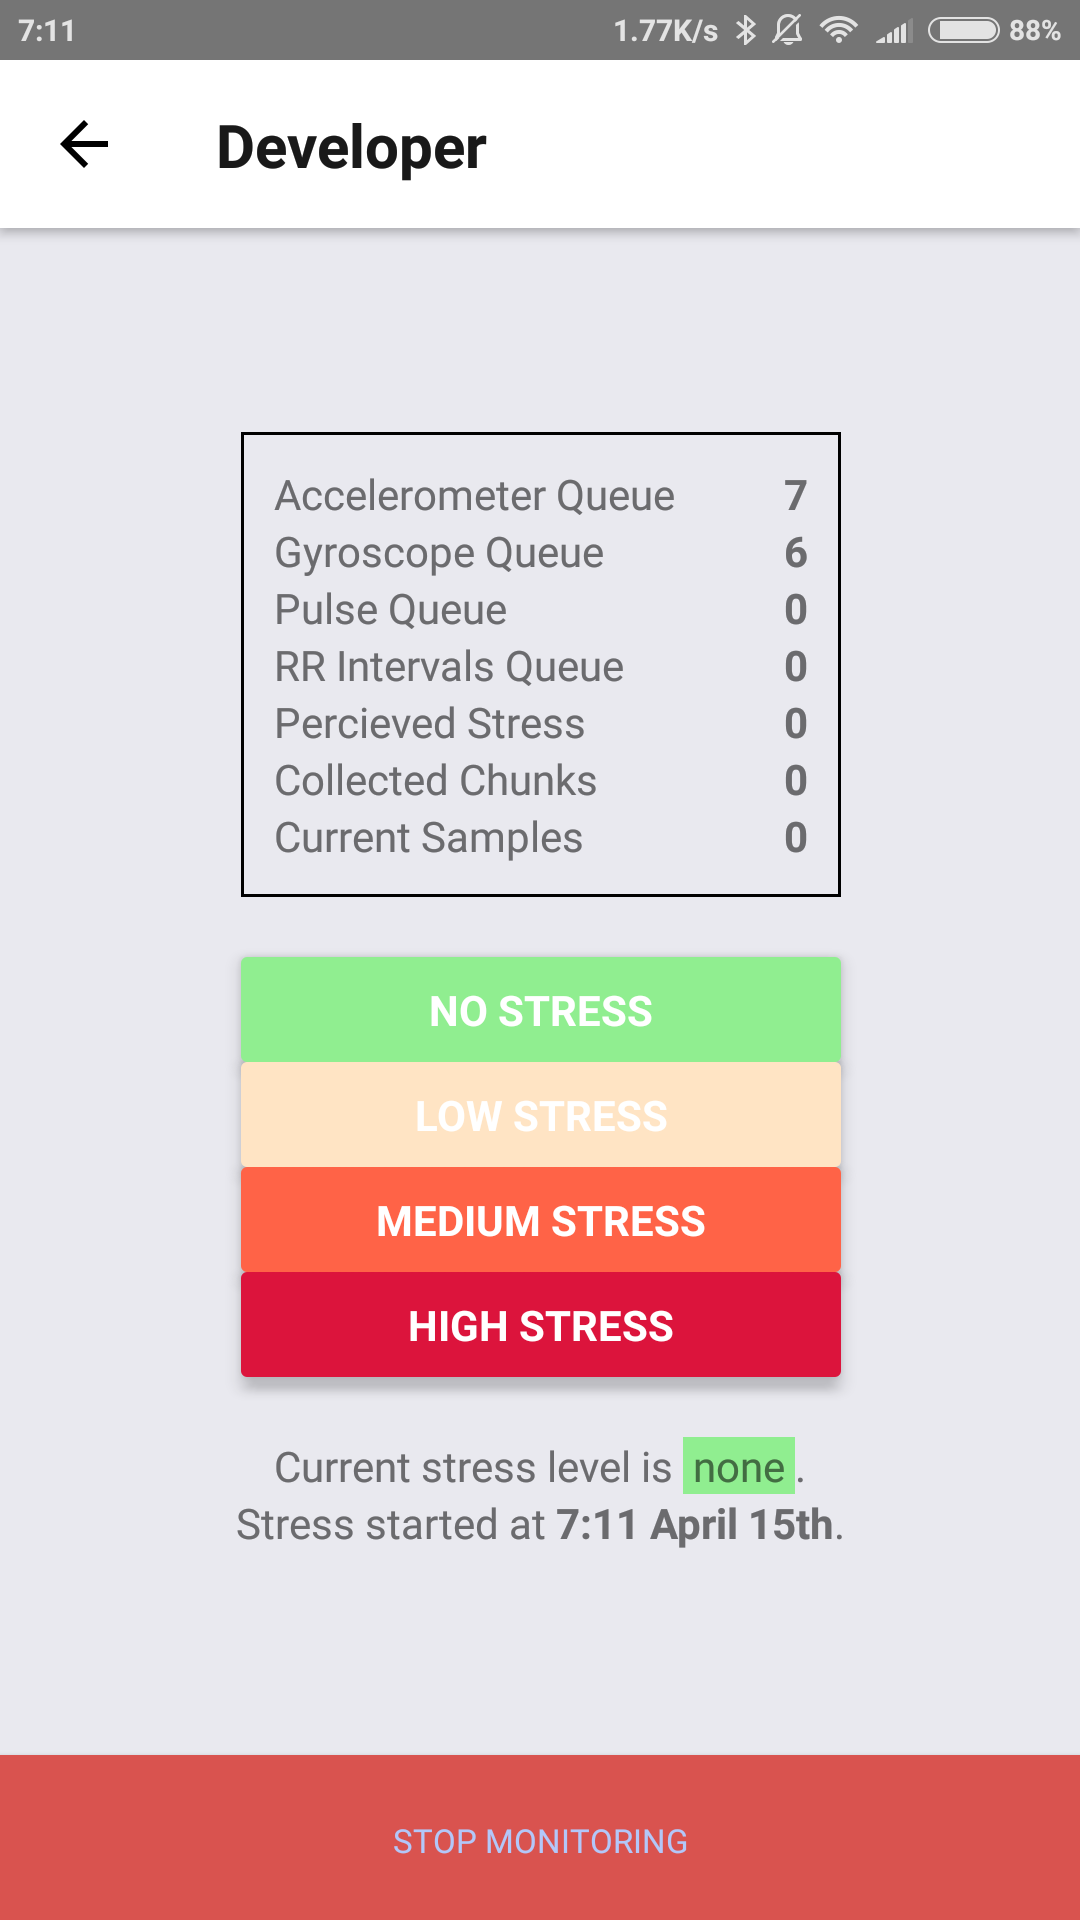
\includegraphics[width=0.4\textwidth]{images/dev.png}
      \label{screenshot:dev}
    }
  \end{center}
	\caption{Экраны приложения}
	\label{screenshots}
\end{figure}

\subsection{Особенности реализации}
Две версии сборки (для разработчика и для пользователя), ...

Ускоренный режим, автоматическая генерация данных, ...

Двухсторонняя очередь для чанков, ...

\section{Модель машинного обучения}
\subsection{Сбор данных}
The Trier social stress test (TSST), ...

Несмотря на бинарную классификацию было принято решение собирать данные о
четырех уровнях стресса. Сделано это было для того, чтобы иметь возможность
более адекватно оценить эффективность модели, не учитывая false positive для
``medium'' стресса и false negative для ``low'' стресса, т.к. ...

\subsection{Тренировка модели}
k-NN, SVM, RandomForest, Naive Bayes, ...

\subsection{Оценка эффективности}
[Комментарий: пока это часть работы не готова, но в конечном итоге тут будут
представлены графики и статистика по false positive и false negative в задаче
классификации.]

\section*{Заключение}
В рамках данной работы был создан прототип мобильного приложения для
автоматического отслеживания человеческого стресса в реальном времени. Показано,
что на основе данных с пульсометра и акселерометра можно эффективно определять
стресс в повседневной жизни. Более детально, были получены следующие результаты:

\begin{itemize}
\item Проанализированы существующие публикации на тему определения стресса на
  основе медицинских данных, выявлены недостатки в их подходах и выбраны
  наиболее важные показатели для определения стресса — вариабельность
  сердцебиения и индекс физической активности.
\item Спроектирована архитектура приложения, позволяющая переиспользовать логику
  обработки данных с медицинских сенсоров во время выполнения и в процессе
  тренировки модели, что в свою очередь помогает последовательно и независимо
  друг от друга разрабатывать мобильное приложение и модель машинного обучения.
\item Написано мобильное приложение для сбора данных с возможностью подключить
  пульсометр по bluetooth и отслеживать изменения в сердцебиении и физической
  активности на графике в реальном времени.
\item Собраны данные для тренировки модели и на их основе натренирована SVM
  модель, которая была портирована в JavaScript, чтобы иметь возможность
  вызывать ее из кода приложения во время его выполнения, не отправляя данные во
  внешнюю систему. [Комментарий: несмотря на то, что модель уже интегрирована, я
  все еще подкручиваю ее параметры и подбираю правильные данные, поэтому про
  оценку эффективности я добавлю позже.]
\end{itemize}

\setmonofont[Path=assets/fonts/, UprightFont=*-Regular, BoldFont=*-Bold,
ItalicFont=*-Italic, BoldItalicFont=*-BoldItalic, Mapping=tex-text]{CMUTypewriterText}
\bibliographystyle{assets/utf8gost705u} \bibliography{diploma}
\end{document}
